% In-context recall on holdout 3: production retrieval versus the agent's own searches.
\begin{figure}[htbp]
\centering
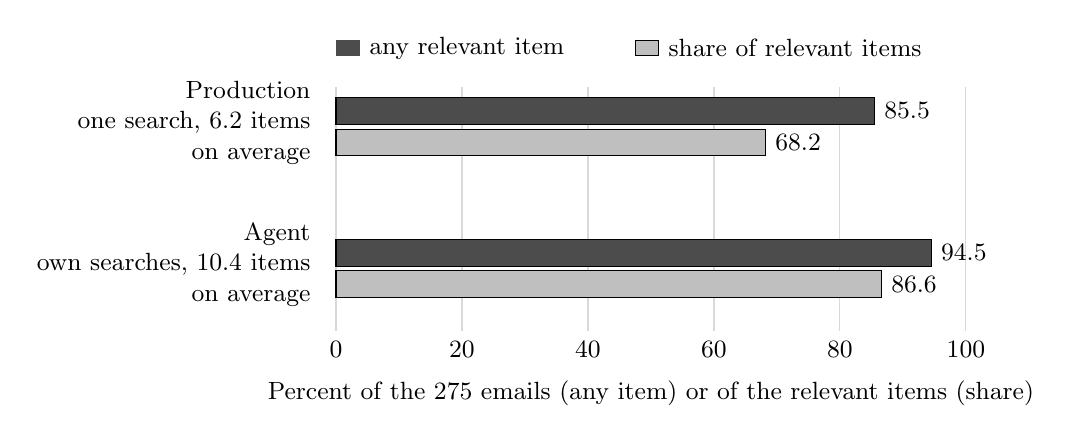
\begin{tikzpicture}[x=1cm,y=1cm,font=\small]
  \foreach \p in {0,20,40,60,80,100} {
    \draw[black!15] ({\p*0.08},0.6) -- ({\p*0.08},-2.5);
    \node[below] at ({\p*0.08},-2.5) {\p};
  }
  \node[below] at (4,-3.0) {Percent of the 275 emails (any item) or of the relevant items (share)};
  \node[left,align=right] at (-0.2,0.15) {Production\\one search, 6.2 items\\on average};
  \node[left,align=right] at (-0.2,-1.65) {Agent\\own searches, 10.4 items\\on average};
  \foreach \y/\v/\f in {0.3/85.5/black!70, -0.1/68.2/black!25, -1.5/94.5/black!70, -1.9/86.6/black!25} {
    \fill[\f,draw=black] (0,\y-0.17) rectangle ({\v*0.08},\y+0.17);
    \node[right] at ({\v*0.08},\y) {\v};
  }
  \fill[black!70] (0,1.0) rectangle (0.3,1.2);
  \node[right] at (0.3,1.1) {any relevant item};
  \fill[black!25,draw=black] (3.8,1.0) rectangle (4.1,1.2);
  \node[right] at (4.1,1.1) {share of relevant items};
\end{tikzpicture}
\caption[Relevant knowledge in the model's context on holdout 3]{Relevant knowledge in the model's context on holdout 3. Production retrieval makes one call on the raw email, and the agent searches about 1.7 times per answer. The dark bars give the percentage of emails with at least one relevant item in context, the light bars the share of all relevant items that reached the context.}
\label{fig:recall-context}
\end{figure}
